
\documentclass{beamer}
\usepackage{graphicx}
%\usepackage{epstopdf}
\usepackage{grffile}
\usepackage{amsmath, amssymb, amsbsy, amstext}
% \usepackage{xcolor}
\usepackage{subfigure}

% \usepackage[utf8]{inputenc}
\usepackage{natbib}

% \usepackage[disable]{todonotes}
\usepackage{todonotes}
\presetkeys{todonotes}{inline}{}

% \usepackage[table]{xcolor}
\usepackage{booktabs} % for much better looking tables
\usepackage{tabularx}

\usepackage{pseudocode}

\usepackage[binary-units]{siunitx}            % For SI units
% \usepackage{enumitem} % control layout of itemize, enumerate, description

\usepackage{pgf}
\usepackage{pgfgantt} % gantt charts

\usepackage{pgfplots}
\pgfplotsset{width=\textwidth,compat=1.9}

% \usepackage{multimedia}
% \usepackage{media9}

\usepackage[export]{adjustbox}[2011/08/13] % for centering wide figures

\usepackage{hyperref}


\newcommand{\code}[1]{{\texttt{#1}}}
\newcommand{\libraryname}[1]{{\texttt{#1}}}
\newcommand{\codefile}[1]{{\textit{#1}}}
\newcommand{\program}[1]{\code{#1}}
\newcommand{\taskname}[1]{{\textit{#1}}}
\newcommand{\newterm}[1]{{\textit{#1}}}
\newcommand{\scarequotes}[1]{`#1'}
\newcommand{\sampleswidth}{0.23\textwidth}
\newcommand{\samplesheight}{1.5cm}
\newcommand{\darwinop}{DARwIn-OP}

% \definecolor{darkgreen}{rgb}{0,0.6,0}
% \logo{\pgfputat{\pgfxy(-2,6)}{\pgfbox[center,base]{\includegraphics[height=2cm]{amsilogo.jpg}}}}

\usetheme[protectframetitle]{m}
% \usetheme{Darmstadt}
% \usetheme{Dresden} %Dresden, Darmstadt, Warsaw
% \usecolortheme{dove}

\newcommand{\ganttslide}[3]{%
\begin{frame}{#1}%
    \begin{figure}[H]%
    % \label{gantt:interim:prelim}
    \centering%
    % \makebox[\textwidth][c]{\resizebox{0.8\paperwidth}{!}{\input{gantt_interim_initial.tex}}}
    \makebox[\textwidth][c]{\resizebox{0.8\paperwidth}{!}{\input{gantt_interim_#2.tex}}}%
    \caption[Project Schedule] {#3}%
  \end{figure}%
\end{frame}%
}


% \title{Optimisation of ball handling behaviour in humanoid robot soccer}
% \title{\vspace{-2.0cm}Biped walk stability improvement for a small humanoid robot}
% \subtitle{COMP4120 research presentation}
% \author{Mitchell Metcalfe}

\title{A Study on Detecting Three-Dimensional Balls using Boosted Classifiers}
% \subtitle{COMP4240 project presentation}
\author{Mitchell Metcalfe, Brendan Annable, Monica Olejniczak, Stephan K. Chalup}
\institute{The University of Newcastle, Australia}
% \date{\today}

% \date{\today \\[1.5\baselineskip] Supervised by Dr. Alex Mendes}
% \date{\today \\[1.5\baselineskip] Supervised by Dr. Alex Mendes}

\begin{document}

\maketitle

\begin{frame}{Outline}
    \tableofcontents
\end{frame}

% a) an introduction to the topic studied
\section{Background and motivation}
\begin{frame}{Robot Soccer}
	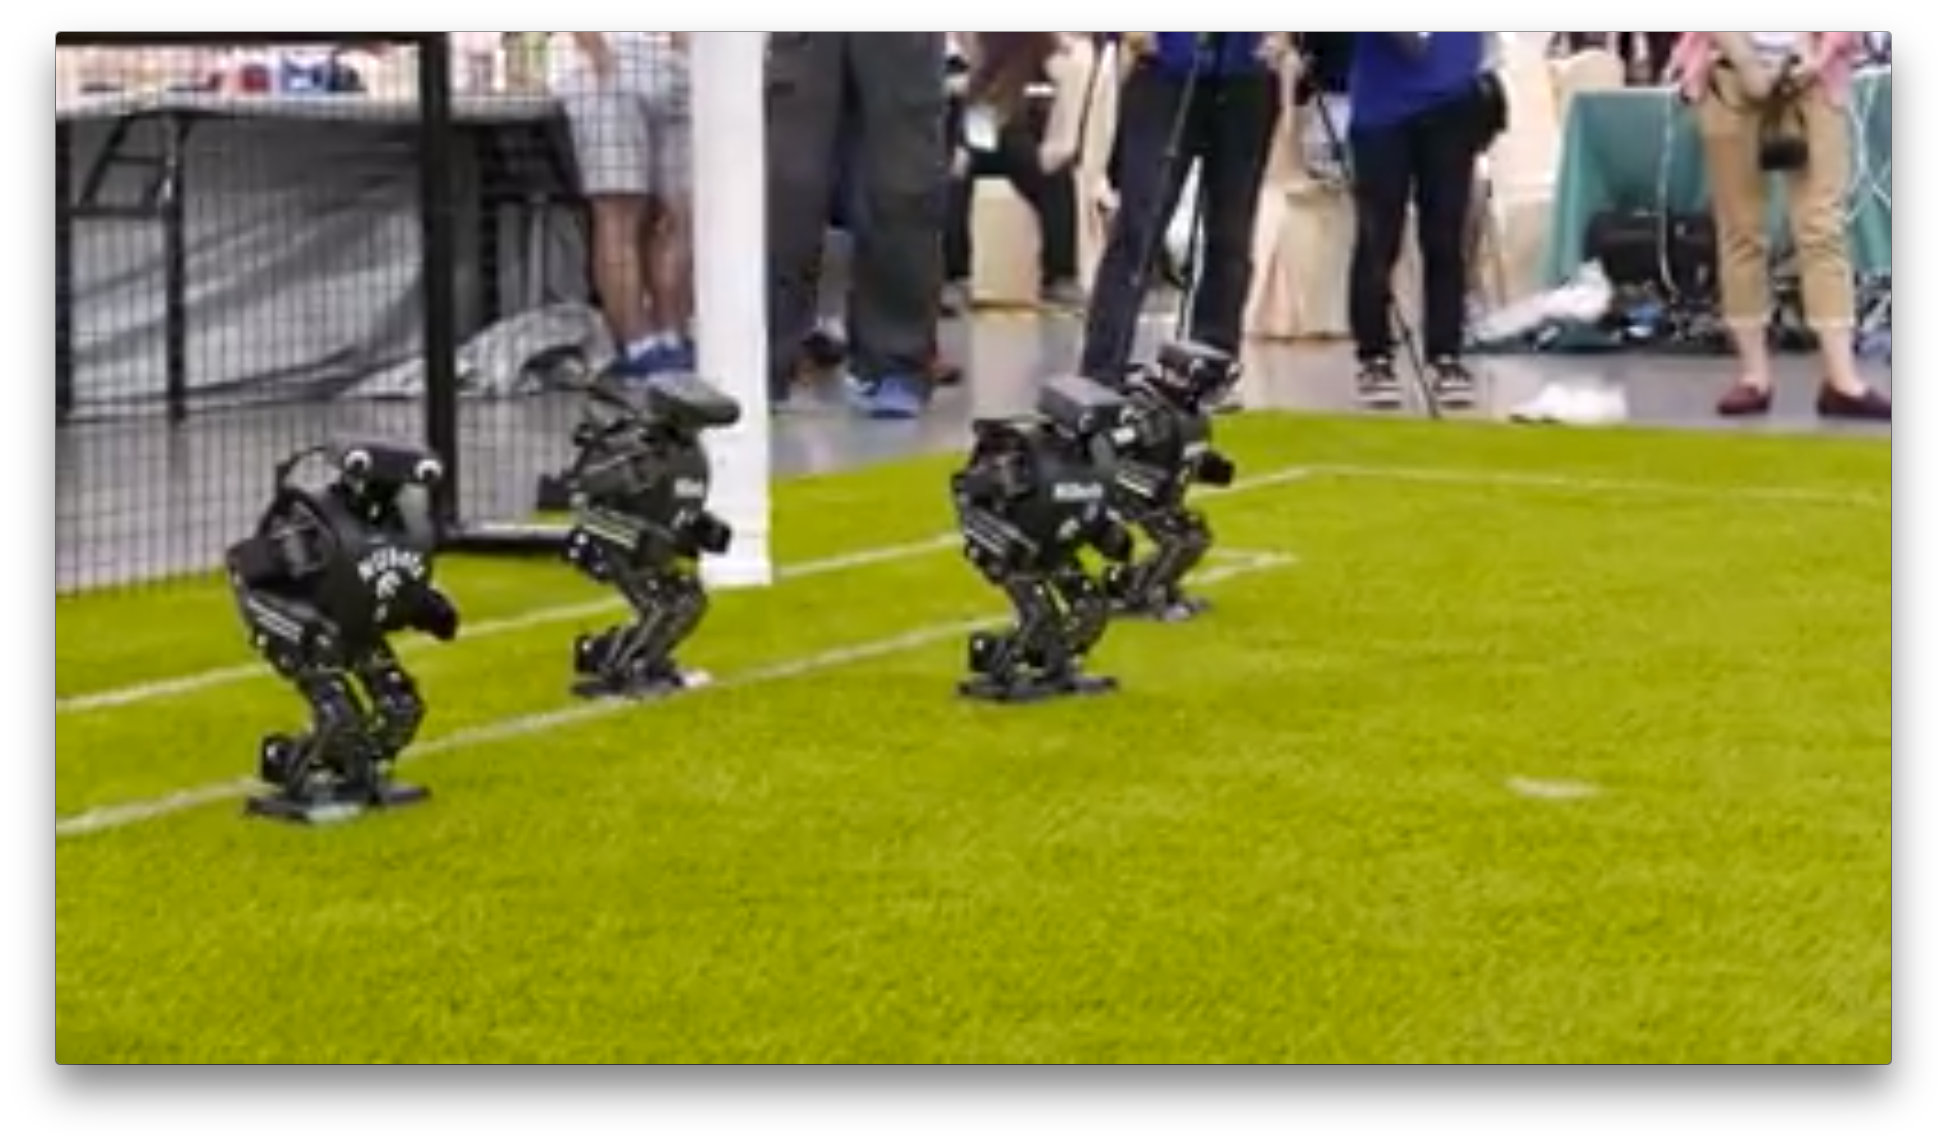
\includegraphics[height=0.6\textwidth]{nubots-first-frame.png}
	% \begin{itemize}
	% 	% \item (Include photo of robots)
	% 	\item Robot soccer team
	% 	\item Competes at RoboCup
	% 	\item Fully autonomous robots
	% 	\item Need to detect and track the ball to play soccer
	% 	\item Have a webcam
	% \end{itemize}
\end{frame}

\begin{frame}{Ball detection}
	Robots at RoboCup \citep{KitanoAKNO97} need to find the ball.
	A common approach is simple circle detection, which has problems: % \par
	% \begin{itemize}
	% 	\item Centre circle
	% 	\item Penalty spots
	% 	\item Line intersections
	% 	\item Anything that looks round from some angle
	% \end{itemize}
	% \begin{center}
	% 	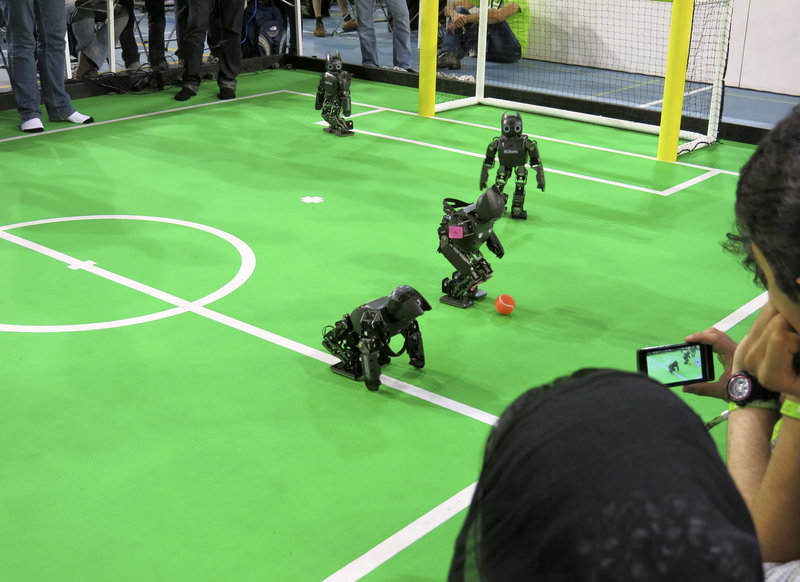
\includegraphics[height=3cm]{field2}
	% \end{center}

	\begin{columns}
		\column{0.5\linewidth}
		\begin{itemize}
			\item Centre circle
			\item Penalty spots
			\item Line intersections
			\item Anything that looks round from some angle
		\end{itemize}
		\column{0.5\linewidth}
			 \centering
			 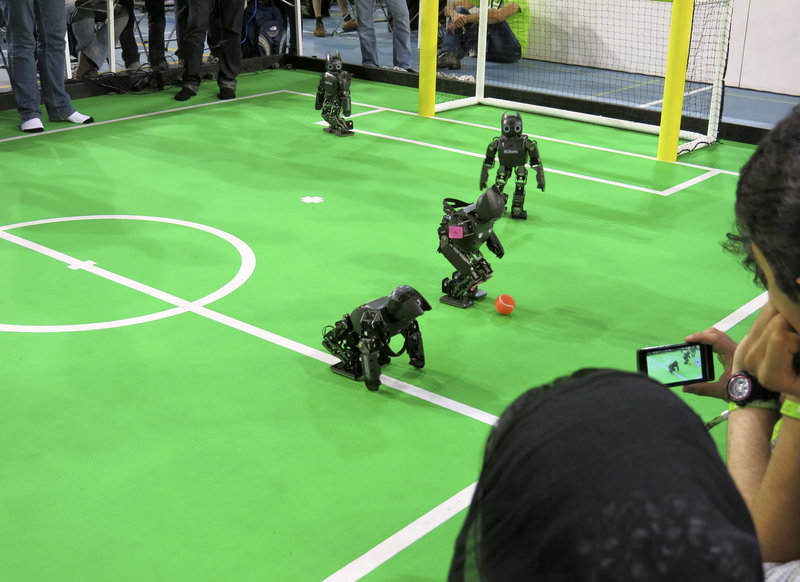
\includegraphics[width=\linewidth]{field2}
			% Robots at RoboCup \citep{KitanoAKNO97} need find the ball.
			% A common approach is simple circle detection, which has problems: % \par
	\end{columns}
\end{frame}

% TODO: Consider removing.
\begin{frame}{Current methods}
	\begin{itemize}
		\item Colour based-methods:
			\begin{itemize}
				\item histogramming
				\item blob-detection
			\end{itemize}
		\item Shape based methods:
			\begin{itemize}
				\item Neural network
				\item Hough filters
				\item RANSAC
			\end{itemize}
		\item Assumptions/limitations:
			\begin{itemize}
				\item Colour classification
					\begin{itemize}
						\item False positives from similarly coloured objects
						\item Unexpected changes in lighting
					\end{itemize}
				\item Circle/Ellipse detection:
					\begin{itemize}
						\item False positives due to disk-like objects in the environment, or objects that appear circular from some angles
					\end{itemize}
			\end{itemize}
	\end{itemize}
\end{frame}

\begin{frame}{Sphere detection}
	% To avoid the limitations of methods based on assumptions such as these, we developed a sphere detection method which uses the shading patterns characteristic of spherical objects to classify objects as spheres.
	More general approach:
	\begin{itemize}
		\item Want to detect differently textured spheres
		\item 3D shading features of spheres have similar spatial constraints to facial features
		\item Investigate the application of techniques popularised in the realm of face detection to the task of sphere detection
	\end{itemize}
\end{frame}

% \begin{frame}{Shading features}
% 	As a result of targeting our approach toward the 3D features that distinguish 3-dimensional balls from objects such as disks, our method is expected to be particularly robust against detecting false positives.
% \end{frame}

% \begin{frame}{Boosted cascade classifiers}
% 	\begin{itemize}
% 		\item Detector must be robust to differently textured spheres
% 		\item  investigated the application of techniques popularised in the realm of face detection to the task of sphere detection
% 		\item 3D shading features of spheres have similar spatial constraints to facial features
% 	\end{itemize}
% % 			\item We assumed that the balls to be detected are resting on the ground and are illuminated from above to constrain the likely positions of shadows and specular highlights.
% \end{frame}

\subsection{Face detection}
\begin{frame}{Face detection}
	\citet{viola2001robust}
	\begin{itemize}
		\item Adaboost: Many \newterm{weak classifiers} `vote' to form a strong classifier
		\item Haar features: Compare the sum of pixel values in two image regions
		\item Detection cascade: Train multiple classifiers that are run in sequence. Allows rejecting false positives quickly.
	\end{itemize}
\end{frame}

\begin{frame}{Similar approaches}
	\citet{nillius2008shading}
	shading based sphere detection using Principal Component Analysis (PCA) with a basis derived analytically from a given Bidirectional Reflectance Distribution Function (BRDF) and assumptions on scene illumination.
	\begin{itemize}
		\item works well for untextured spheres
		\item does not work well for spheres with patterns
	\end{itemize}
\end{frame}

\begin{frame}{Ball detection approaches}
	% \begin{itemize}
		% \item
		\citet{masselli2013haar}
			\begin{itemize}
				\item Used a boosted Haar cascade classifier
				\item Outperformed a Hough transform based approach
				\item Tested on uniformly yellow, green, and white balls
			\end{itemize}
		% \item A similar approach [21] attempted to detect a wide variety of generic FIFA-style balls by using extended Haar features as weak classifiers.
	% \end{itemize}
\end{frame}

\begin{frame}{Ball detection approaches}
	\citet{zhang2013novel}
	\begin{itemize}
		\item Used modified Haar features
		\item Improved performance
	\end{itemize}
	% reported improved performance when modified Haar features that used a division operation between their area sums, instead of the usual subtraction, were included. This suggests that exploring alternate weak classifiers could lead to valuable performance improvements.
\end{frame}

\begin{frame}{Ball detection approaches}
	\citet{mitri2004fast}
	\begin{itemize}
		\item Performed training and classification on `edge image'
		% \item Preprocessed samples using a Sobel filter and a threshold function to each image as preprocessing steps
		% \item learn Classification and Regression Trees (CARTs) of Haar features
		\item Performs well for ball tracking, but detected other round objects as false positives
		% \item Performed better when a more complex training dataset was applied%, which included images under different lighting conditions and environments.
		\item Poor false positive rate may be due to ignoring shading information% of the spheres by using only an edge image.
\end{itemize}
\end{frame}

\begin{frame}{Ball detection approaches}
	\citet{treptow2004filter}
	\begin{itemize}
		\item Low false positive rate using a boosted Haar-cascade
		\item Only attempt to classify a single type of soccer ball
	\end{itemize}
\end{frame}

\section{Hypothesis}
\begin{frame}{Hypothesis}
	Including a large proportion of disk-like negative images in the training set will increase the precision of the resulting sphere detectors.
\end{frame}

\section{Dataset}
\begin{frame}{ImageNet \citep{imagenet_cvpr09}}
	All training and testing images were sourced from ImageNet.
	% \begin{itemize}
	% 	\item Image database for computer vision
	% 	\item organised according to the WordNet hierarchy
	% 	\item some images have associated bounding box information
	% \end{itemize}

	Prior to training, each sample is:
	\begin{itemize}
		\item cropped from its original image
		\item resized to 24x24 pixels
		\item converted to grayscale
	\end{itemize}

	Set aside a random 20\% of the samples for use as a test set.
\end{frame}
% \begin{frame}{Positive and Hard Negative samples}
% 	\begin{itemize}
% 		\item images from ImageNet that have bounding box information
% 		\item Prior to training, each sample is:
% 			\begin{itemize}
% 				\item cropped from its original image
% 				\item resized to 24x24 pixels
% 				\item converted to grayscale
% 			\end{itemize}
% 	\end{itemize}
% \end{frame}
% \begin{frame}{WordNet categories (‘synsets') used}
% 	\begin{itemize}
% 			\item Positive
% 			\item Negative
% 			\item Background
% % 				\item (explain what a background image is)
% 			\item A randomly selected 20\% of the samples of each of the two sample sets was set aside for use as a test set before beginning training.
% 	\end{itemize}
% \end{frame}

\begin{frame}{Positive categories}
\begin{table}[t]
	\centering
	\caption{ImageNet synsets used for the positive samples in the training set and their associated WordNet identifiers.}
	\label{tab:positive_samples}
	\begin{tabularx}{1.0\columnwidth}{@{}lX@{}}
		\toprule
		\textbf{Id} & \textbf{Name} \\
		\midrule
			n02778669 & Ball \\
			n02779435 & Ball \\
			n02799071 & Baseball \\
			n03131967 & Cricket ball \\
			n03445777 & Golf ball \\
			n13899404 & Ball, globe, orb \\
		\bottomrule
	\end{tabularx}
\end{table}
\end{frame}

\begin{frame}{Blacklisted categories}
\begin{table}[h]
	\centering
	\caption{Blacklisted ImageNet synsets and their associated WordNet identifiers.}
	\label{tab:blacklisted_synsets}
	\begin{tabularx}{1.0\columnwidth}{@{}lX@{}}
	\toprule
	\textbf{Id} & \textbf{Name} \\
	\midrule
	n04023962 & Punching bag, punch bag, punching ball, punchball \\
	n04118538 & Rugby ball \\
	n04186051 & Shaving cream, shaving soap \\
	n09229709 & Bubble \\
	\bottomrule
	\end{tabularx}
\end{table}
\end{frame}

\begin{frame}{Background categories}
\begin{table}[t]
	\centering
	\caption{ImageNet synsets used for the background samples in the training set and their associated WordNet identifiers.}
		\label{tab:background_samples}
	\begin{tabularx}{1.0\columnwidth}{@{}lX@{}}
	\toprule
	\textbf{Id} & \textbf{Name} \\
	\midrule
	n02782778 & Ballpark, park \\
	n02913152 & Building, edifice \\
	n03841666 & Office, business office \\
	n04335209 & Street \\
	n08524735 & City, metropolis, urban center \\
	n08659446 & Field \\
	\bottomrule
	\end{tabularx}
\end{table}
\end{frame}

\begin{frame}{Negative categories}
\begin{table}[t]
	\centering
	\caption{ImageNet synsets used for the negative samples in the training set and their associated WordNet identifiers.}
		\label{tab:negative_samples}
	\begin{tabularx}{1.0\columnwidth}{@{}lX@{}}
	\toprule
	\textbf{Id} & \textbf{Name} \\
	\midrule
	n03032811 & Circle, round \\
	n13873502 & Circle \\
	n13873917 & Circle \\
	n13875185 & Disk, disc, saucer \\
	n13875392 & Ring, halo, annulus, doughnut, anchor ring \\
	n13875970 & Coil, whorl, roll, curl, curlicue, ringlet, gyre, scroll \\
	n13902336 & Rim \\
	\bottomrule
	\end{tabularx}
\end{table}
\end{frame}

\begin{frame}{Additional negative samples}
	\begin{itemize}
			\item ELSD (Ellipse and Line Segment Detector) \citep{Patraucean:2012jf}
			\item Detect ellipses in background images
			\item Create samples using bounding boxes around each ellipse
			% \item Only use near-complete ellipses
	\end{itemize}
\end{frame}

% \begin{frame}{Background training set}
% 	\begin{itemize}
% 		\item randomly sample one square window from each background image
% 		\item side lengths between 20\% and 100\% of image size
% 	\end{itemize}
% \end{frame}

\newcommand{\samplefigurewidth}{0.45\textwidth}
\newcommand{\samplewidth}{0.14\textwidth}
\newcommand{\sampleheight}{0.14\textwidth}
\newcommand{\includesample}[1]{\hspace{0.1cm}\includegraphics[width=\samplewidth,height=\sampleheight]{images/training/#1}}

\begin{frame}{Example samples}
	\begin{figure}[h]
		\centering
		\subfigure[Positive samples.]{%
			% Enclose in shortstack to enable line break.
			\shortstack{%
				% Positive
				\includesample{positive/positive_1}%
				\includesample{positive/positive_2}%
				\includesample{positive/positive_3} \\%
				% Positive thumbnails
				\includesample{positive/positive_1_thumbnail}%
				\includesample{positive/positive_2_thumbnail}%
				\includesample{positive/positive_3_thumbnail}%
			}%
			\label{fig:positive_samples}%
		}%
		\qquad
		\subfigure[Hard negative samples.]{%
			% Enclose in shortstack to enable line break.
			\shortstack{%
				% Hard negative
				\includesample{hard_negative/hard_negative_1}%
				\includesample{hard_negative/hard_negative_2}%
				\includesample{hard_negative/hard_negative_3} \\%
				% Hard negative thumbnails
				\includesample{hard_negative/hard_negative_1_thumbnail}%
				\includesample{hard_negative/hard_negative_2_thumbnail}%
				\includesample{hard_negative/hard_negative_3_thumbnail}%
			}%
			\label{fig:negative_samples}%
		}%
		% \caption{Examples of positive (a) and hard negative (b) samples used for training. The first row represents the original image, while the second row represents the same samples that have been cropped, resized and converted to grayscale prior to training.}
		\label{fig:samples}
	\end{figure}
\end{frame}

\section{Experiment}
\begin{frame}{Experiment}
	\begin{itemize}
		\item Train Viola-Jones detector cascades \citep{viola2001robust}
		\item Use two different feature types:
			\begin{itemize}
				\item Extended Haar features \citep{Lienhart2002extended}
				\item Local Binary Patterns (LBPs) \citep{liao2007learning}
			\end{itemize}
	\end{itemize}
\end{frame}

\begin{frame}{Summary of trials}
	% 	\item Summary of trials:
	% 		\begin{itemize}
	% 			\item Training set size: 9300
	% 			\item Positive \%: 40
	% 			\item Hard Neg \%: \{0, 10, 20, 30, 40, 50\}
	% 			\item NumPos: 200
	% 			\item NumNeg: 350
	% 			\item Feature type: \{HAAR, LBP\}
	% 		\end{itemize}
	% \end{itemize}

	\begin{table}
		\centering
		\caption{A summary of the 12 experimental trials}
		\label{tab:training_schemes}
		% \scalebox{0.8}{
		\begin{tabularx}{\columnwidth}{@{}rX@{}}
			\toprule
			\textbf{Parameter} & \textbf{Value} \\
			\midrule
	{Set size}     & 9300 \\
	{Pos. \%}      & 40 \\
	{Hard Neg. \%} & \{0, 10, 20, 30, 40, 50\} \\
	{NumPos}       & 200 \\
	{NumNeg}       & 350 \\
	{Feature type} & \{Haar, LBP\} \\
			\bottomrule
		\end{tabularx}
		% }
	\end{table}
\end{frame}


\section{Results}

\begin{frame}{Results: Recall}
	\begin{figure}
		\centering
		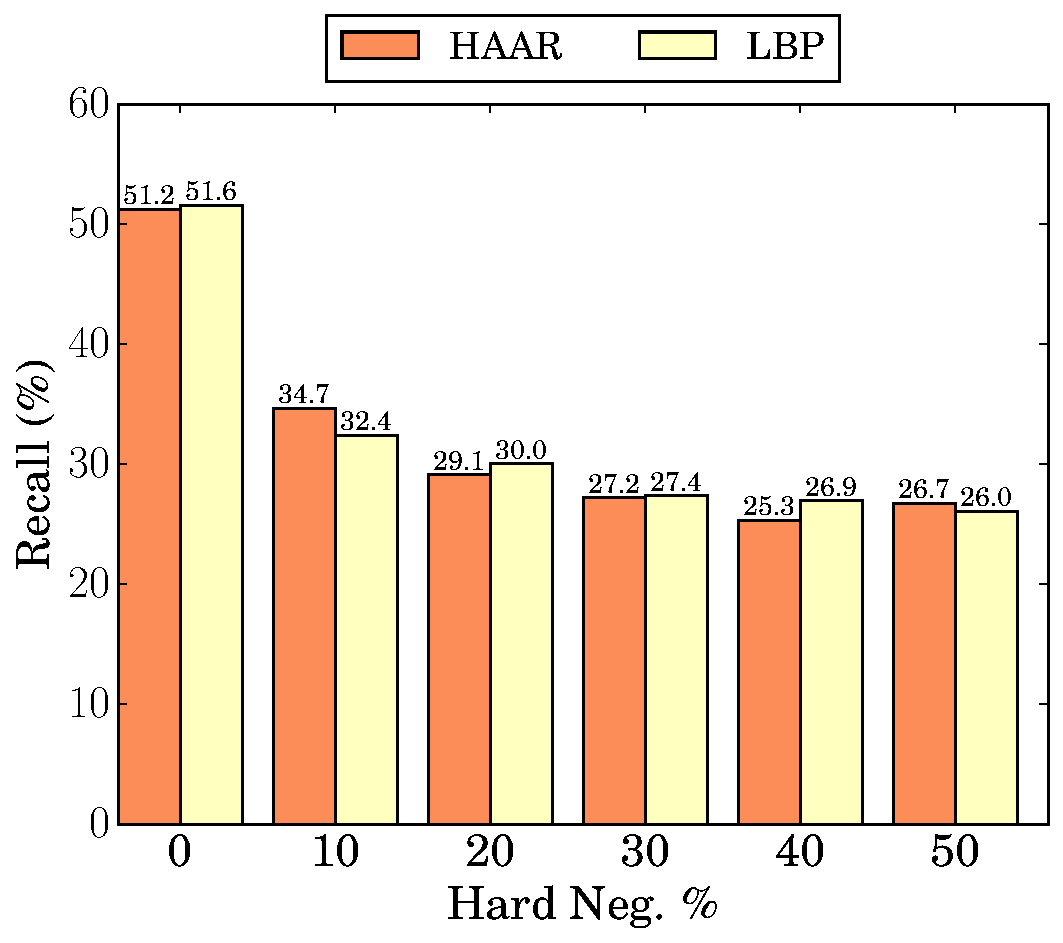
\includegraphics[width=0.73\textwidth]{results/results_fig_recall_6.pdf}%
	\end{figure}
\end{frame}
\begin{frame}{Results: Precision}
	\begin{figure}
		\centering
		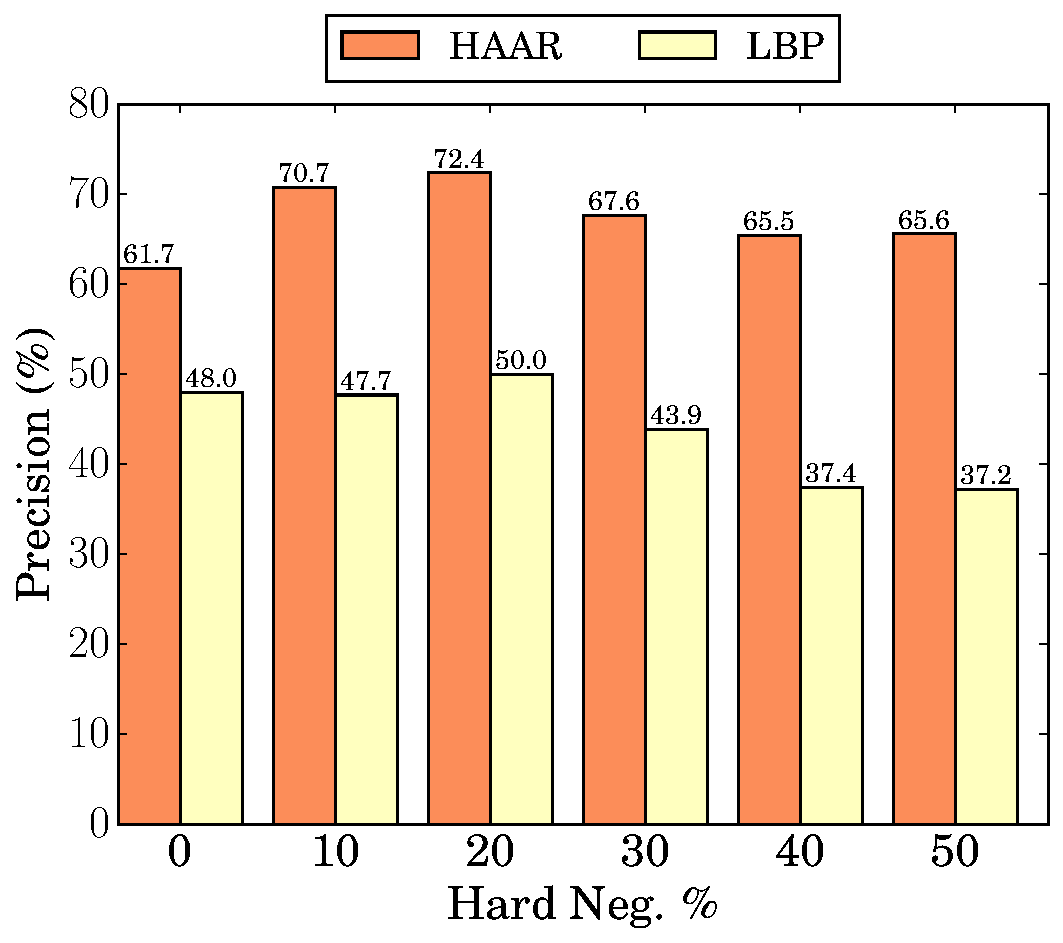
\includegraphics[width=0.73\textwidth]{results/results_fig_precision_6.pdf}%
	\end{figure}
\end{frame}

\begin{frame}{Results}
	\begin{figure}
		\centering
		% \qquad
		\subfigure{%
		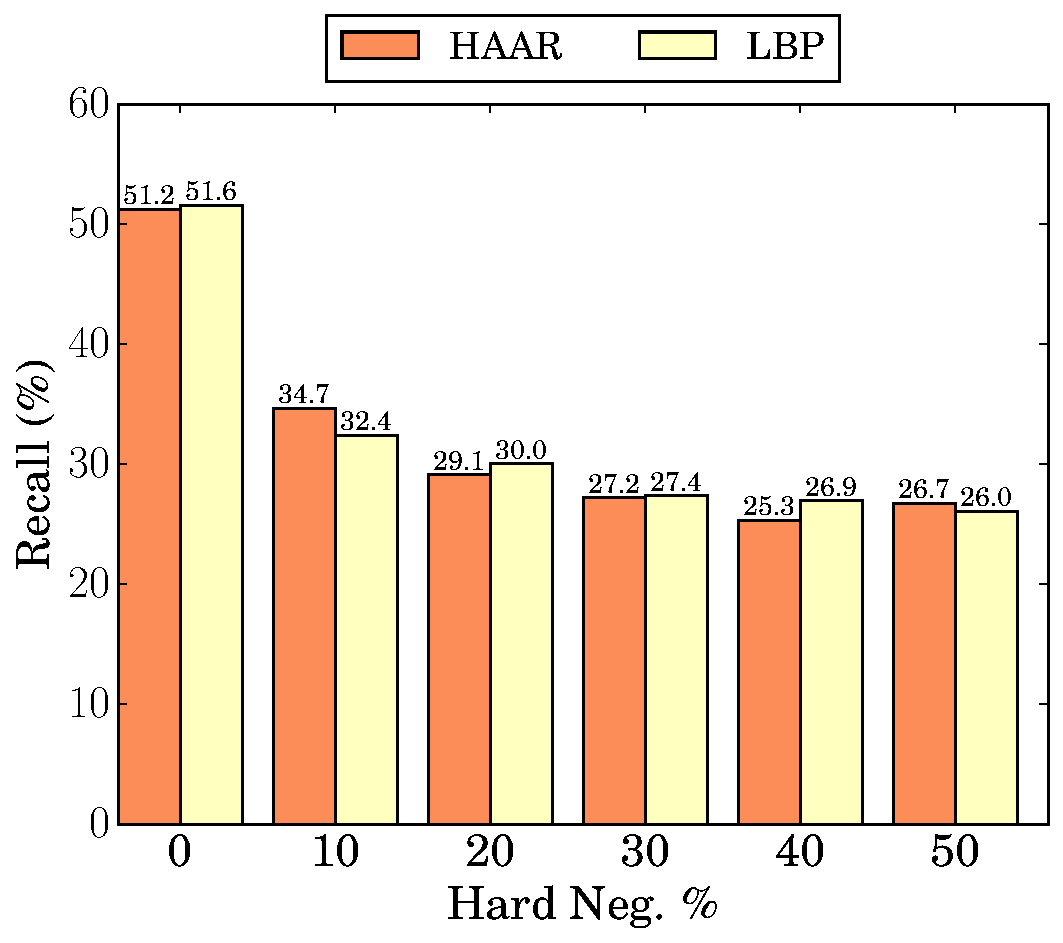
\includegraphics[width=0.5\textwidth]{results/results_fig_recall_6.pdf}%
		\label{fig:trial_comparison_chart_recall}%
		}%
		\subfigure{%
		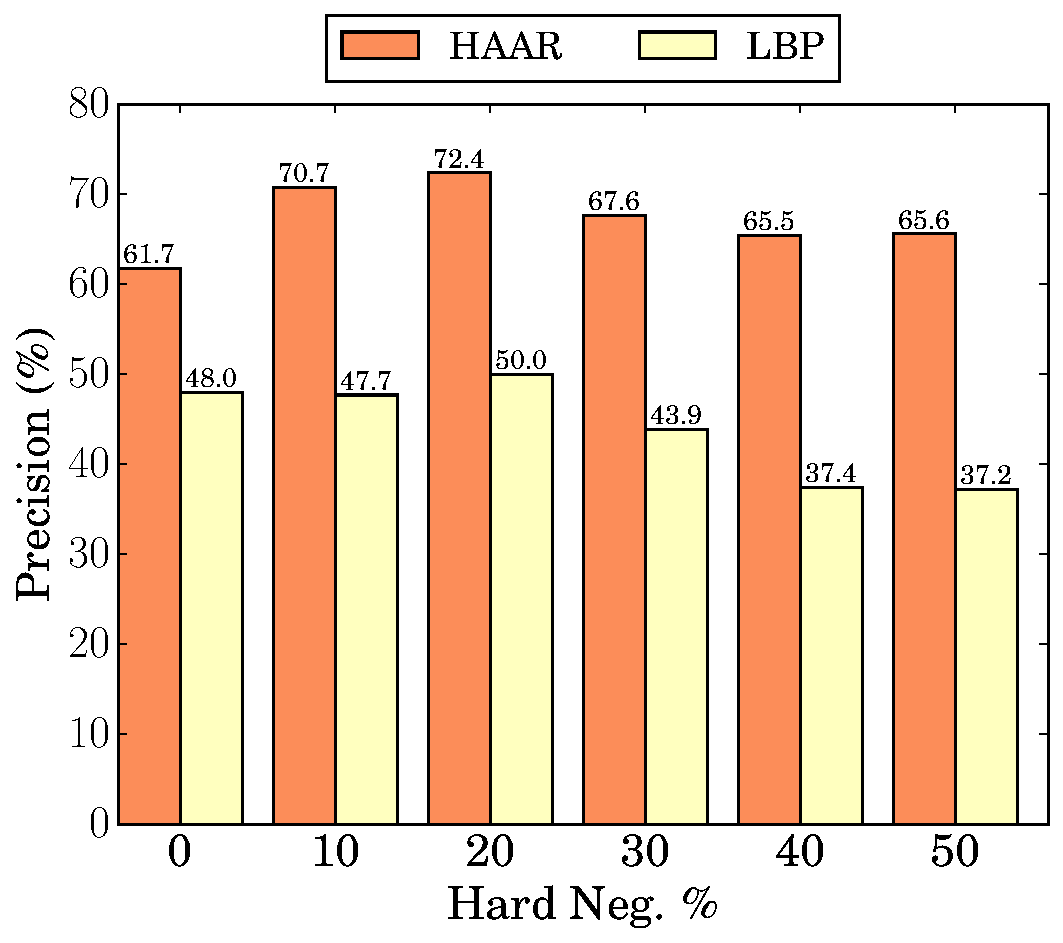
\includegraphics[width=0.5\textwidth]{results/results_fig_precision_6.pdf}%
		\label{fig:trial_comparison_chart_precision}%
		}%
		% \caption{Column graphs comparing the proportion of the negative samples in the training set of each trial that were `hard negatives' (images of round, non-spherical objects) with the resulting rates of precision and recall.}
		\label{fig:trial_comparison_charts}
	\end{figure}
\end{frame}

\begin{frame}{Live detection performance}
	\begin{figure}
	  \centering
	  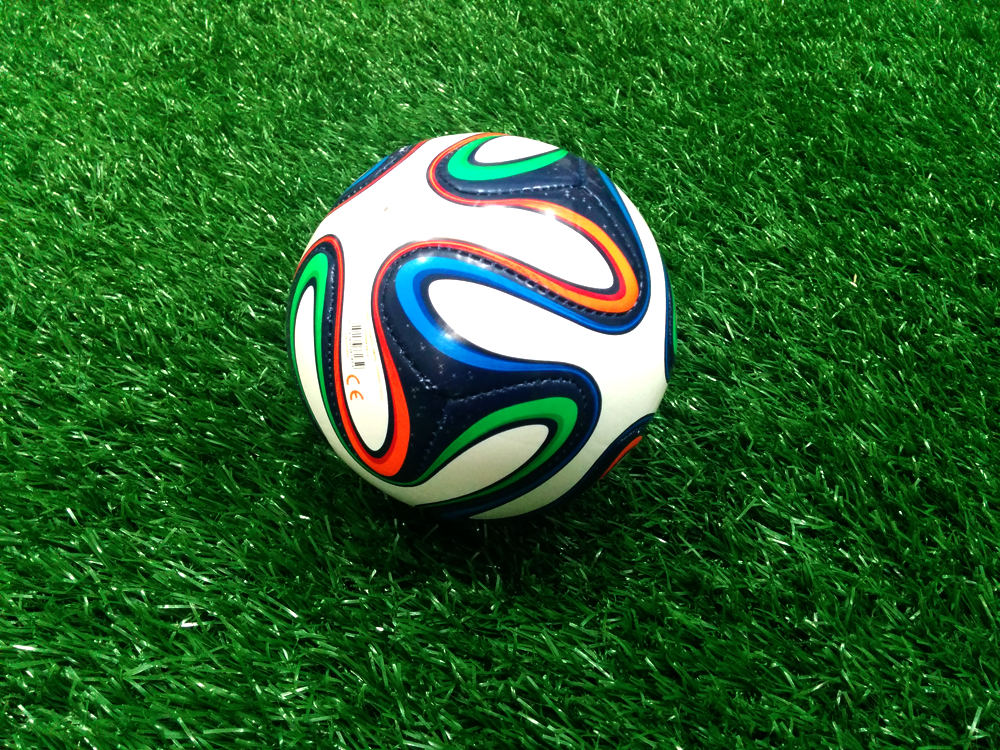
\includegraphics[width=0.7\textwidth]{images/fifa_ball}
	%   \caption{Ball that often could not be detected.}
	  \label{fig:fifa_ball}
	\end{figure}
\end{frame}

\newcommand{\includesequence}[1]{\includegraphics[width=0.2\textwidth]{images/rotation/#1}}

\begin{frame}{Live detection performance}
	\begin{figure}
	  \centering
	  \begin{tabularx}{1.0\textwidth}{@{}XXXXX@{}}
		\includesequence{2}  &
			\includesequence{25} &
			\includesequence{31} &
			\includesequence{35} &
			\includesequence{39} \\
			\includesequence{43} &
			\includesequence{53} &
			\includesequence{59} &
			\includesequence{64} &
			\includesequence{74} \\
	  \end{tabularx}
	%   \caption{Sequence of rotated webcam images. In the training data it was assumed that natural light usually comes from above. The displayed results indicate that the ball detector uses the geometric positioning of shadows and highlights as a characteristic feature that is common to 3D balls.}
	  \label{fig:rotated_sequence}
	\end{figure}
\end{frame}

\section{Conclusion}

	\begin{frame}{Summary of results}
		\begin{itemize}
			\item Haar > LBP, for sphere detection
			\item The results for classifiers using Haar features support the hypothesis
		\end{itemize}
	\end{frame}

	\begin{frame}{Interactive entertainment}
		% Robust 3D object detection will also be important for developers of interactive entertainment applications, such as augmented reality games and networked exergames, where remote players may interact with real objects such as balls [13].
		\begin{itemize}
			\item Augmented reality
			\item Telepresence
			\item Highlight real objects
		\end{itemize}
	\end{frame}

    \begin{frame}{Bibliography}
      \vspace{-2em}
      \bibliographystyle{apalike}
    %   \scriptsize
      \fontsize{0.5em}{0.5em}\selectfont
      \bibliography{bibliography}
    \end{frame}

    % \plain{Questions?}

\end{document}
